\chapter{Infeasibility Gliding in Compositional Spaces} \label{chap:infeasibilitygliding}

A

\begin{figure}[h]
    \centering
    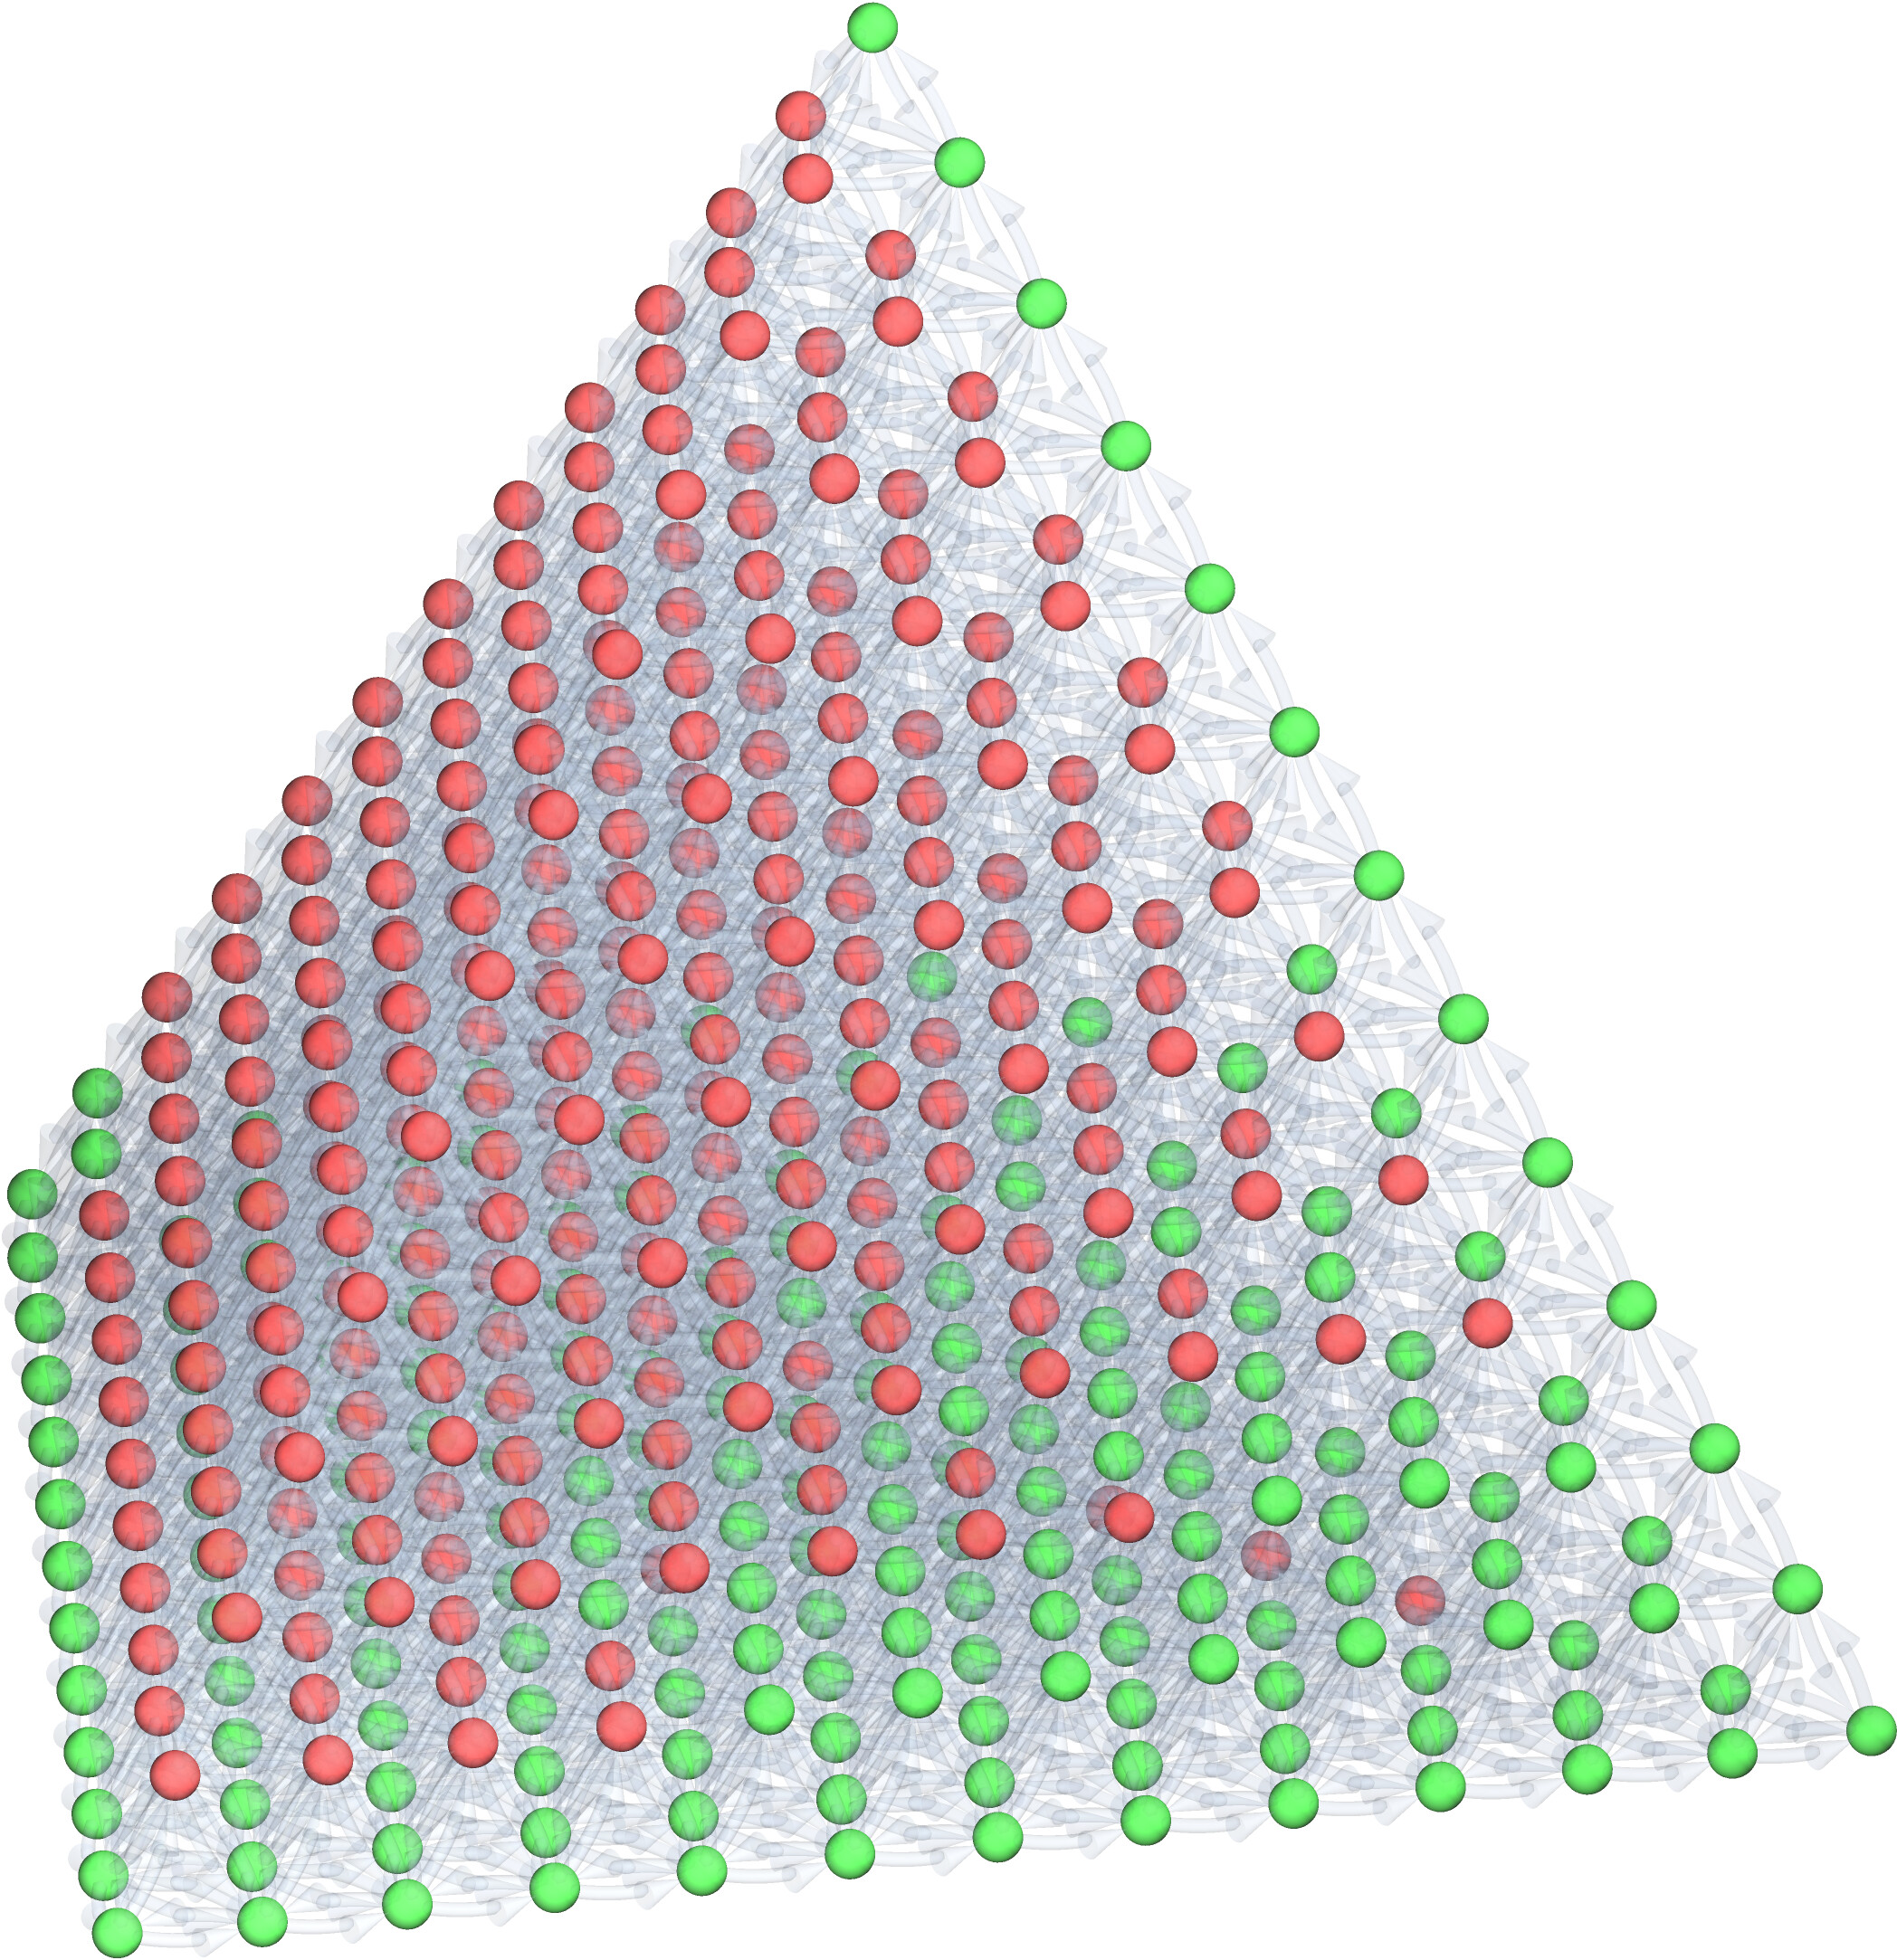
\includegraphics[width=0.7\textwidth]{infeasibilitygliding/InfeasibilityGliding_Full.png}
    \caption{Feasibility map over compositional tetrahedron (3-simplex) formed by all combinations of Ti50 Zr50, Hf95 Ti5, Mo33 Nb33 Ta33, Mo80 Nb10 W10 discretized at 12 divisions per dimension. The positions in the 7-component elemental space obtained from \texttt{nimplex}, described in Chapter \ref{chap:nimplex}, were used to run \texttt{pycalphad} \cite{Otis2017Pycalphad:Python} evaluations and constrained by limiting phases present at equilibrium at 1000K to single or many solid solution phases. Roughly half of the compositions are infeasible with most of them forming a single large region.}
    \label{fig:fullcomputation}
\end{figure}

B

\begin{figure}[h]
    \centering
    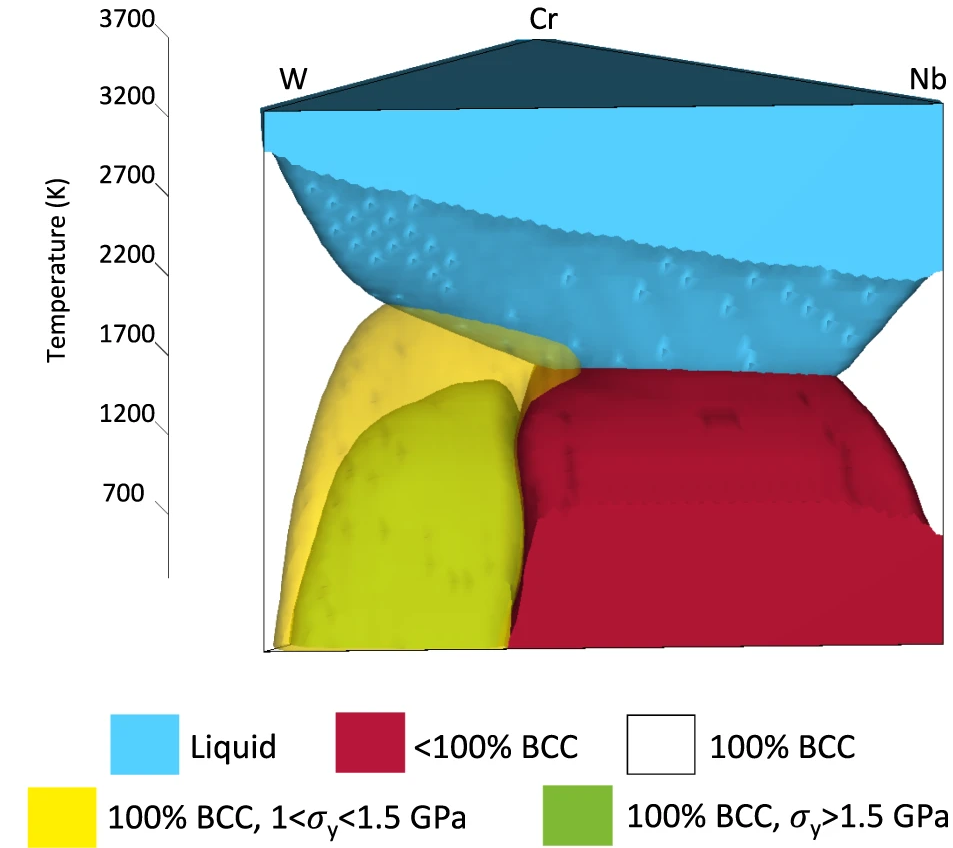
\includegraphics[width=0.8\textwidth]{infeasibilitygliding/PhaseTernaryMap_Elder2023.png}
    \caption{A view of ternary Cr-Nb-W phase diagram projected across a temperature range of phase classes, further augmented by imposing predicted property value constraints. It depicts the smoothness of the infeasible region boundary (red) and increasingly smooth boundary of property-constrained region. Taken from Figure 2b in \citet{Elder2023ComputationalValidation} under CC BY 4.0 license.}
    \label{fig:katesphasemap}
\end{figure}

C

\begin{figure}[h]
    \centering
    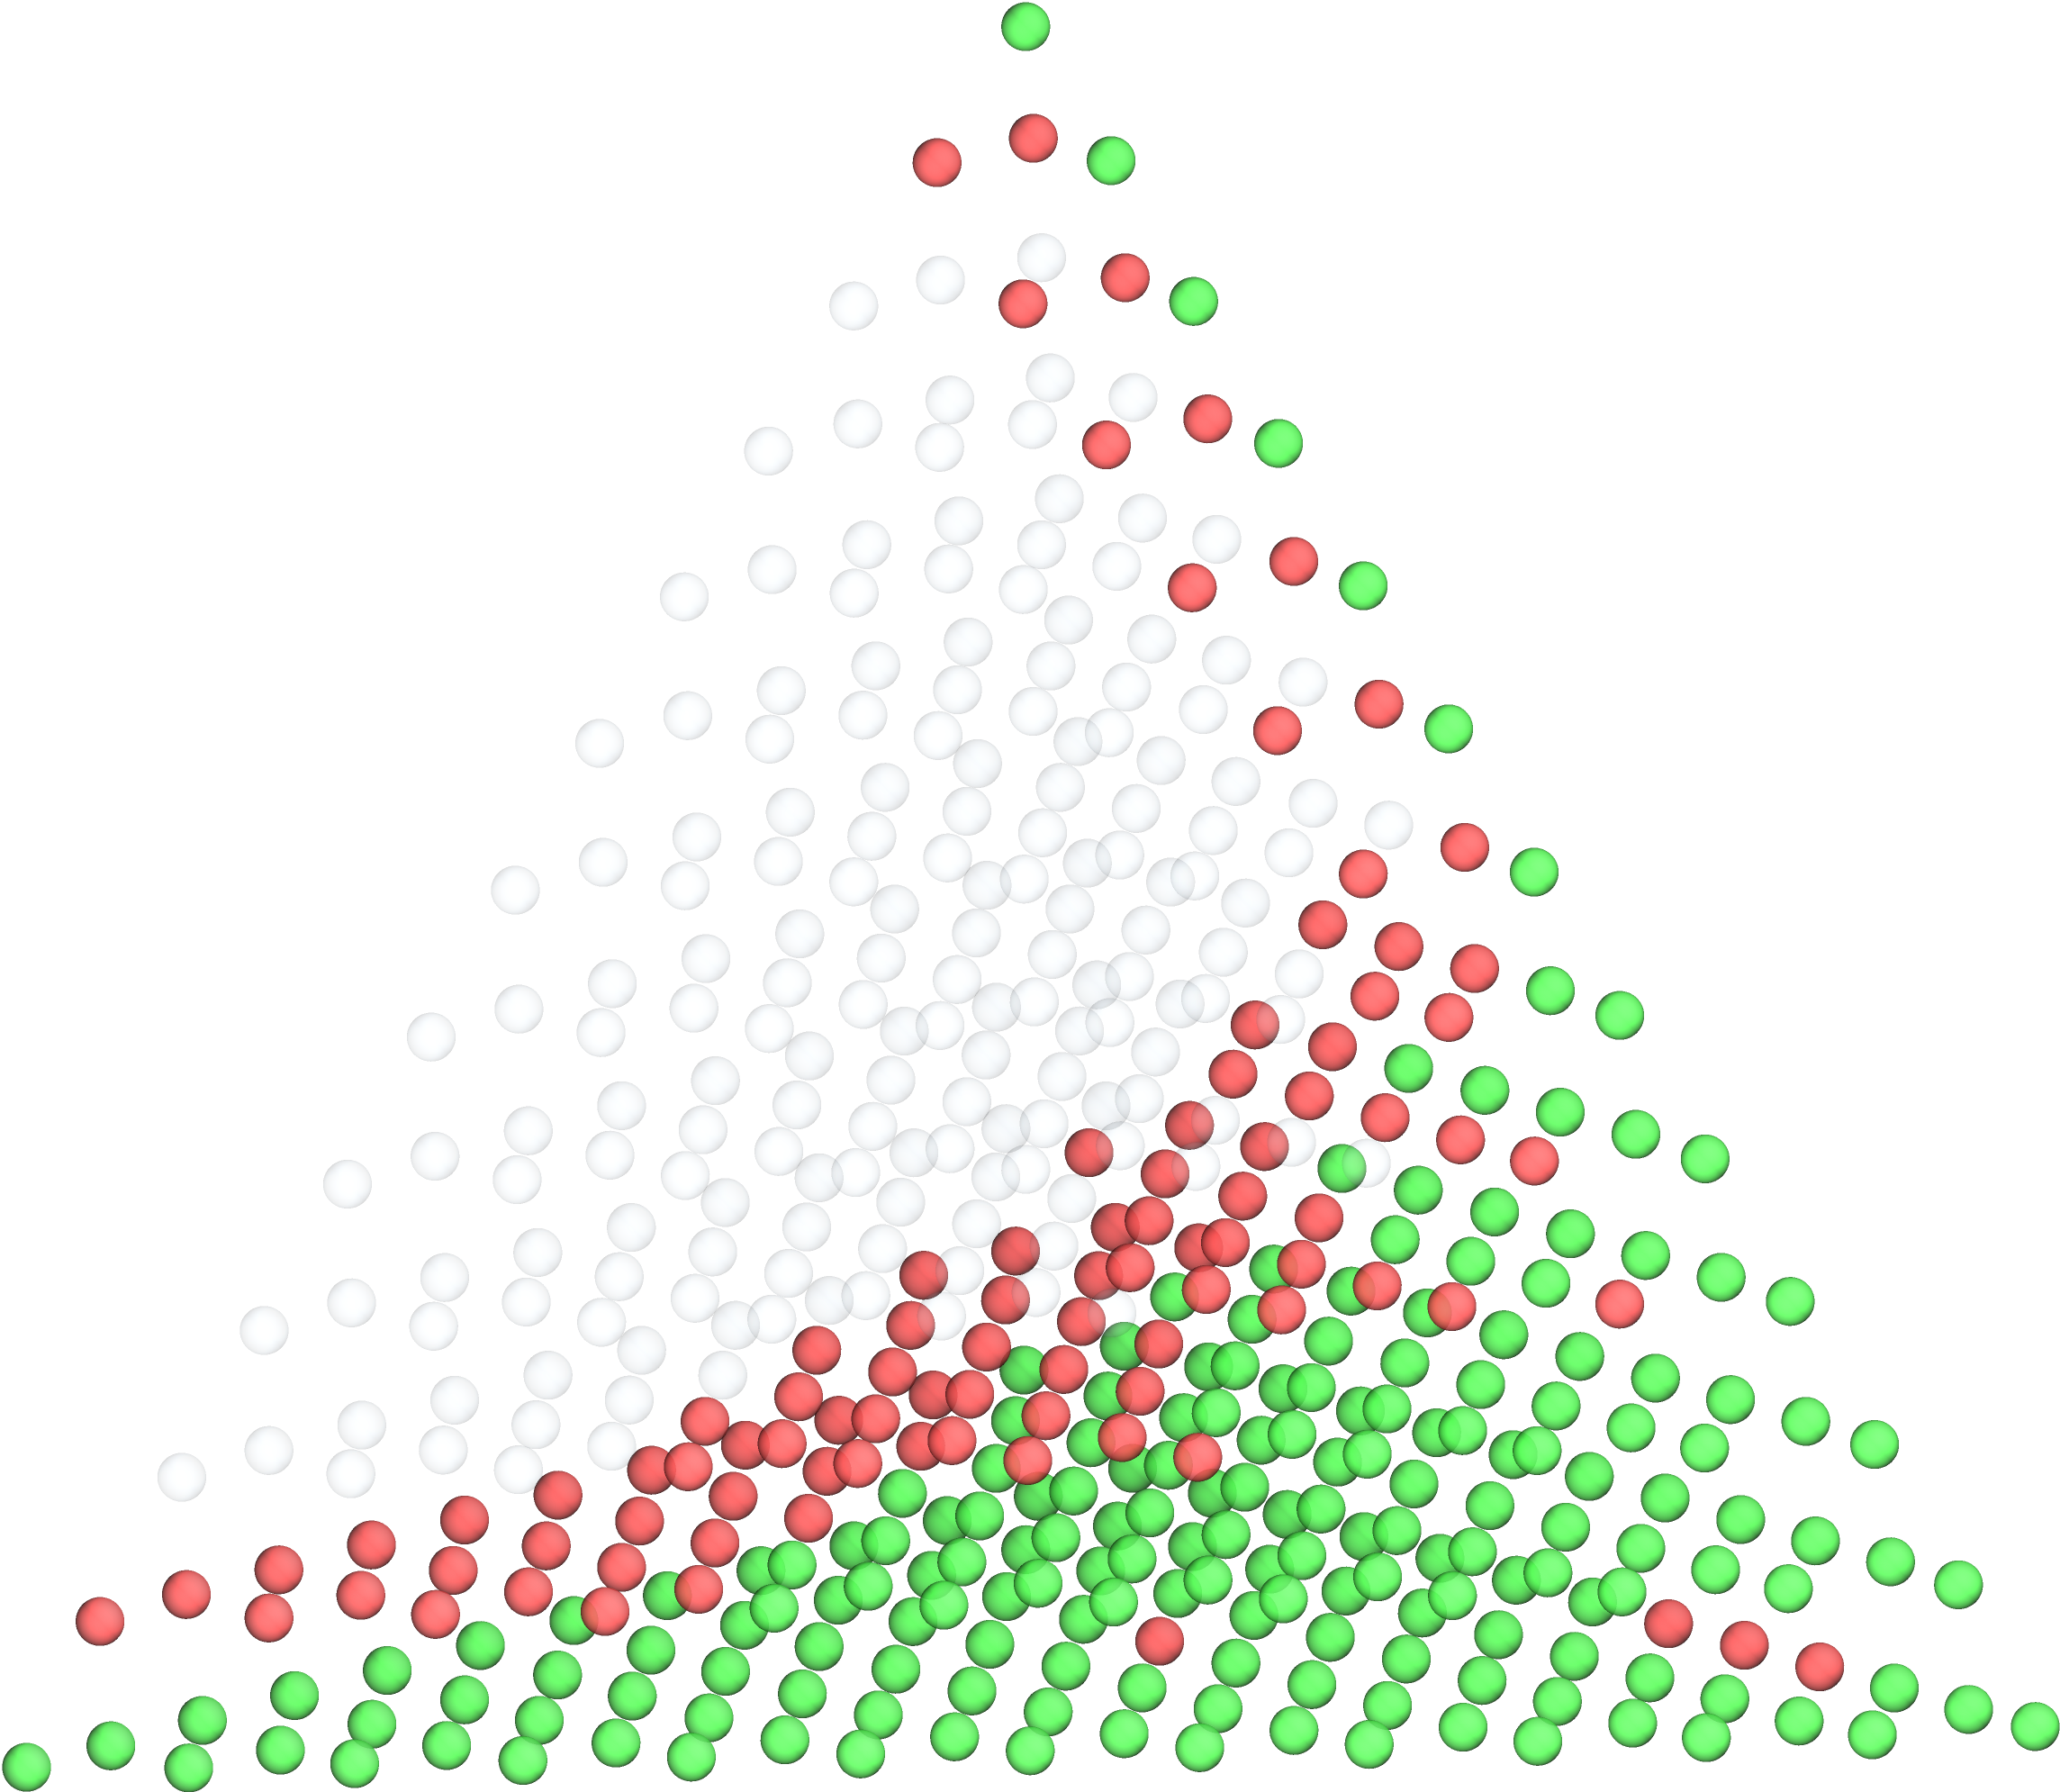
\includegraphics[width=0.7\textwidth]{infeasibilitygliding/InfeasibilityGliding_Glide.png}
    \caption{The same problem as in Figure \ref{fig:fullcomputation} solved by iteratively exploring all feasible paths in the compositional graph in depth-first approach, which can be started from one or multiple points, and terminated once goal is reached or once all of the feasible space is explored.}
    \label{fig:glide}
\end{figure}


\printbibliography[heading=subbibintoc]